% Title: Area Under a Curve (AUC) Module
% Author: Jason Regina
% Date: 12 May 2016
% Description: Documentation for OnRamp AUC module

% Document options
\documentclass[a4paper, 11pt]{article}

% Header options
\usepackage{fancyhdr}
\pagestyle{fancy}
\fancyhf{}
\rhead{\small Area Under a Curve}
\lhead{\small OnRamp Module}
\rfoot{\small Page \thepage}

% Image options
\usepackage{graphicx}
\usepackage{float}
\usepackage{wrapfig}
\graphicspath{{images/}}
\usepackage[labelfont=bf]{caption}

% Font options
\usepackage{mathpazo}
\linespread{1.05}
\usepackage[scaled]{helvet}
\usepackage{courier}
\normalfont
\usepackage[T1]{fontenc}
\usepackage{microtype}
\usepackage{url}
\urlstyle{same}
\usepackage{algpseudocode}
\usepackage{algorithm}

% Table options
\usepackage{booktabs}
\usepackage{array}
\usepackage{tabu}
\renewcommand{\arraystretch}{1.5}

% Title options
\usepackage{titling}

\makeatletter
\title{\textbf{Area Under a Curve}}
\author{\textsc{Jason Regina}\\
{\textit{University of Wyoming}}}
\date{\today}

% Change the square brackets for each bibliography item from '[1]' to '1.'
\renewcommand\@biblabel[1]{\textbf{#1.}}

% Reduce the space between items in the itemize and enumerate environments and the bibliography
\renewcommand{\@listI}{\itemsep=0pt}

% Decimal section numbers
\renewcommand*\thesection{\arabic{section}.0}
\renewcommand*\thesubsection{\arabic{section}.\arabic{subsection}}

% Custom title
\renewcommand{\maketitle}
{
	\begin{flushright}
	{\LARGE\@title}

	\vspace{25pt}

	{\large\@author}
	\\\@date

	\end{flushright}
}
\makeatother

%----------------------------------------------------------------------------------------

\begin{document}

% Insert title
\maketitle
\bigskip

%----------------------------------------------------------------------------------------
%	SUMMARY
%----------------------------------------------------------------------------------------

\begin{description}
  \item[Summary] Use a Riemann sum to approximate the area under a curve
  \item[Duration] 3 hours
  \item[Prerequisites] Calculus I or exposure to algebraic summations
\end{description}

%----------------------------------------------------------------------------------------
%	OVERVIEW
%----------------------------------------------------------------------------------------

\section{Overview}

This module introduces a method to approximate the area under a curve using a Riemann sum. Serial and parallel algorithms addressing shared and distributed memory concepts are discussed, as well as the MapReduce algorithm classification. A method to estimate pi ($\pi$) is also developed to demonstrate an example scientific application. Exercises focus on how to measure the performance and scaling of a parallel application in multi-core and many-core environments. 

Upon completion of this module, students should be able to: 1) Understand the importance of approximating the area under a curve in modeling scientific problems, 2) Understand and apply parallel concepts, 3) Measure the scalability of a parallel application over multiple or many cores, and 4) Identify and explain the Area Under a Curve algorithm using the Berkeley Dwarfs system of classification.

Much of the material in this module has been adapted from the Area Under a Curve module written by Aaron Weeden\cite{website:weeden:2015}.

%----------------------------------------------------------------------------------------
%	INTRODUCTION TO THE PROBLEM
%----------------------------------------------------------------------------------------

\section{Approximating the Area Under a Curve}

Calculating the area under a curve is an important task in science. The area under a concentration-time curve is used in neuroscience to study changes in endocrine levels in the body over time. In economics, the area under a curve is used in the study of discounting to determine the fee incurred for delaying a payment over time. Applications of the area under a curve are used in many other fields of science, including machine learning, medicine, psychology, chemistry, and environmental science.

%------------------------------------------------

\subsection{Riemann sums}

Several techniques exist which can be used to provide acceptable approximations for the area under a curve. This module considers the Riemann sum method of integration. A Riemann sum is a summation that takes the form:

\begin{equation}
\label{riemann}
	\sum_{}^{} f(x) \Delta x
\end{equation}

Riemann sums can be used to approximate the area under a curve by dividing the area into multiple component shapes and summing their areas. The specific Riemann method explored in this module involves dividing the domain of integration into several rectangles. The height of an arbitrary rectangle is given by $f(x)$ and the width is $\Delta x$. The sum of the areas of the rectangles formed by this method is the approximation of the area under the curve. This module considers the Left Riemann sum, in which $f(x)$ indicates the height of the left-most side of each rectangle. A pictorial example of the Left Riemann sum is shown in Figure 1.

\begin{figure}[H]
\begin{center}
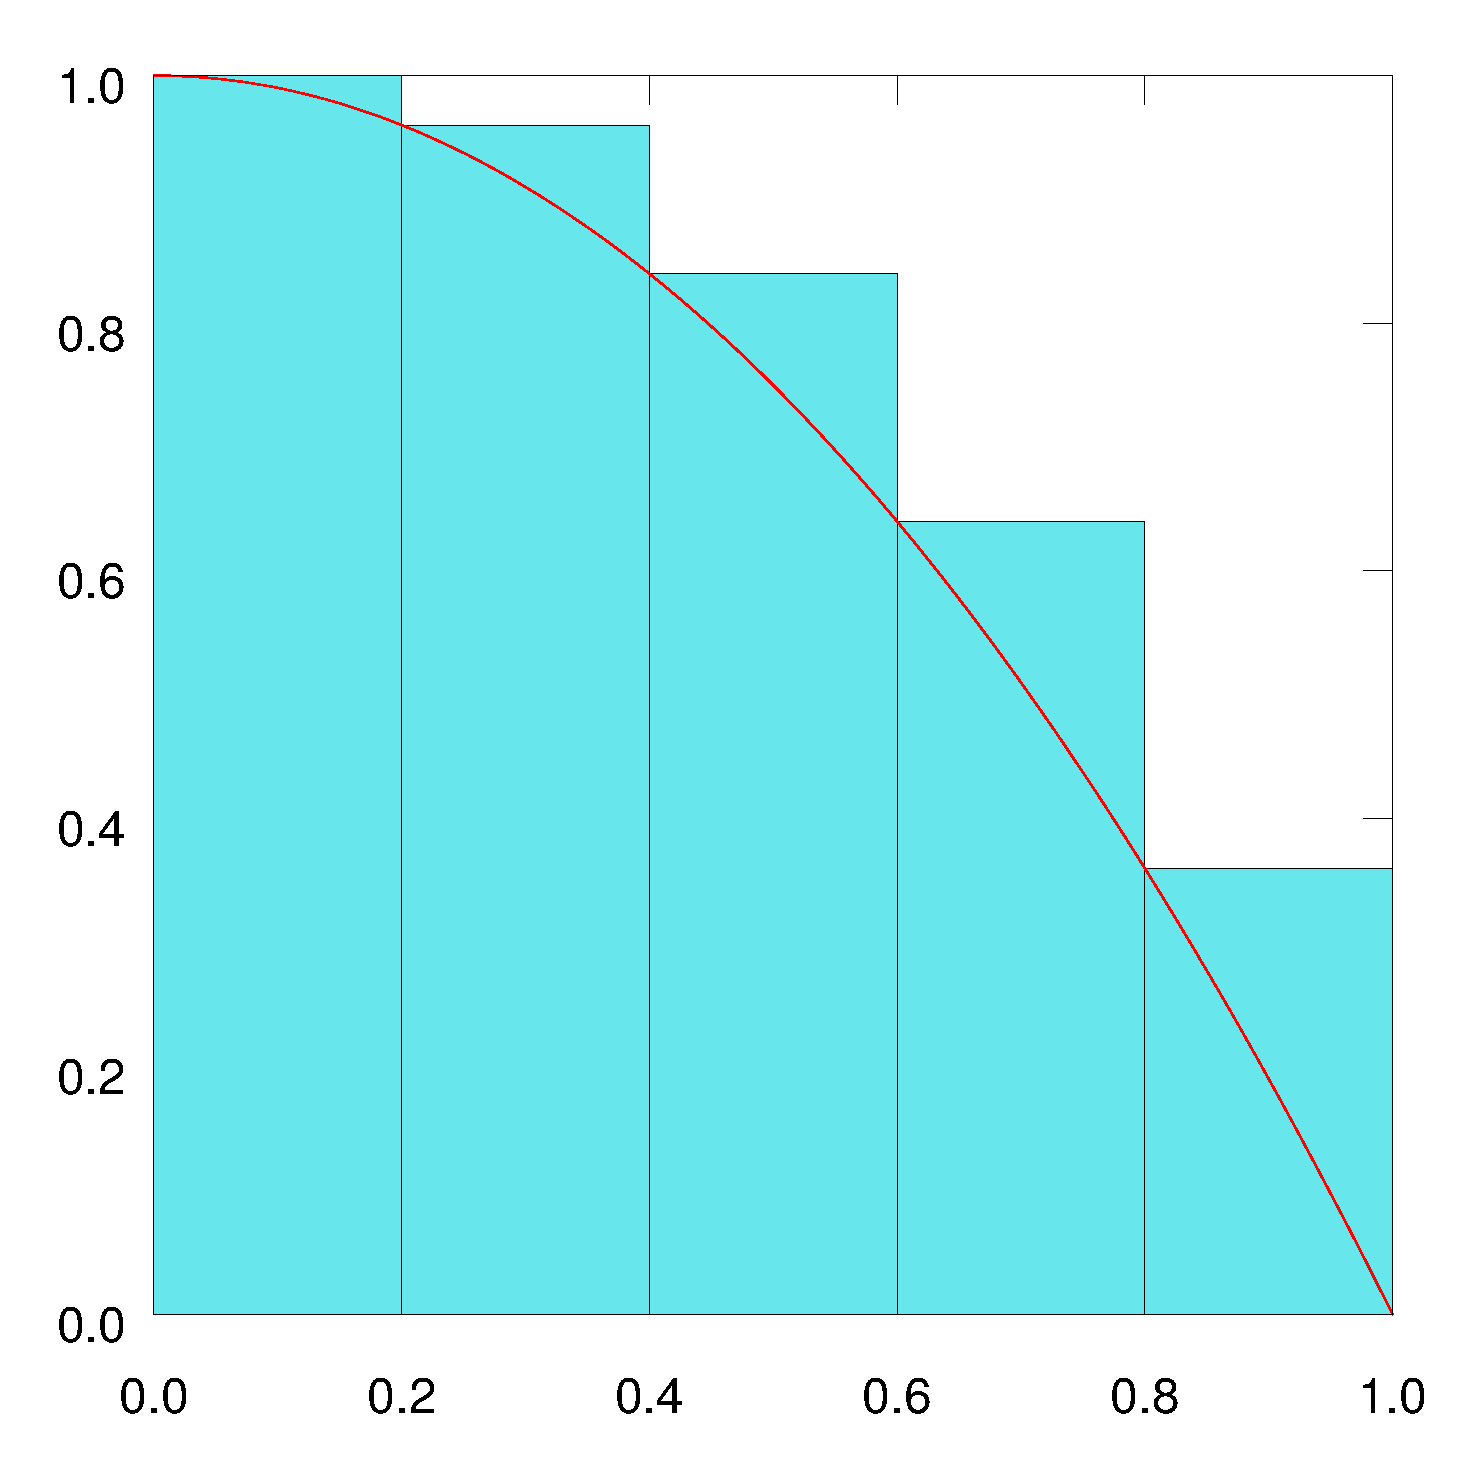
\includegraphics[width=0.5\textwidth]{riemann-sum.pdf} 
\caption{Left Riemann Sum}
\end{center}
\end{figure}

\bigskip
\paragraph{Quick Review Questions}
\begin{enumerate}
\item What does ``left'' refer to in the left Riemann sum?
\item What does ``sum'' refer to in the left Riemann sum?
\end{enumerate}

%------------------------------------------------

\subsection{Estimating Pi in Serial}

A unit circle has a radius of 1.0 and an area of pi. Given a unit circle centered at the origin and limiting the Riemann sum to Quadrant I, pi can be approximated by:

\begin{equation}
\label{pi}
	\pi = 4 \sum_{i=0}^{N-1} (1 - x_{i}^2) \Delta x_{i}\ ,\qquad 0 \leq x < 1
\end{equation}

Where $i$ is the index of an arbitrary rectangle, $N$ is the number of rectangles, $(1 - x_{i}^2)$ is the height of rectangle $i$, and $\Delta x_{i}$ is the width of rectangle $i$.

For a small number of rectangles, calculations can be performed easily by hand or using a calculator. Beyond just a few rectangles, however, the area needs to be approximated using a computer. Many serial (non-parallel) algorithms for approximating the area under a curve exist with many coded implementations. Such code, running on a single computer, can calculate the areas of millions of rectangles in a Riemann sum in a very small amount of time.

A possible implementation of equation 2 written in pseudocode is shown in Algorithm \ref{serial}.

\begin{algorithm}
\caption{Area Under a Curve --- Serial}
\label{serial}
\begin{algorithmic}
\Require $N$
\Ensure $N$ is an integer greater than 0
\State $i\gets 0$ \Comment{Initialize $i$}
\State $PI\gets 0$ \Comment{Initialize $PI$}
\State $\Delta x = 1 / N$ \Comment{Calculate $\Delta x$}
\While{$i < N$} \Comment{Repeat for all rectangles}
\State $x = i / N$ \Comment{Calculate $x$}
\State $area = (1 - x^2) \Delta x$ \Comment{Calculate rectangle $area$}
\State $PI \gets PI + area$ \Comment{Add $area$ to total sum}
\State $i\gets i + 1$ \Comment{Increment $i$}
\EndWhile
\State $PI \gets 4 * PI$ \Comment{Approximate $PI$}
\end{algorithmic}
\end{algorithm}

To approximate with even more rectangles, one needs to employ more processing power than is available on a single processor. The concept of parallel processing can be used to leverage the computational power of computing architectures with multiple or many processors working together.

%----------------------------------------------------------------------------------------
%	INTRODUCTION TO PARALLELISM
%----------------------------------------------------------------------------------------

\section{Introduction to Parallelism}

In parallel processing, rather than having a single program execute tasks in a sequence, the program is split among multiple \emph{execution flows} executing tasks in parallel, i.e. at the same time. The term \emph{execution flow} refers to a discrete computational entity that performs processes autonomously. A common synonym is \emph{execution context}; \emph{flow} is chosen here because it evokes the stream of instructions that each entity processes.

Execution flows have more specific names depending on the flavor of parallelism being utilized. In \emph{distributed memory} parallelism, in which execution flows keep their own private memories (separate from the memories of other execution flows), execution flows are known as \emph{processes}. In order for one process to access the memory of another process, the data must be communicated, commonly by a technique known as \emph{message passing}. The standard of message passing considered in this module is defined by the \emph{Message Passing Interface (MPI)}, which defines a set of primitives for packaging up data and sending them between processes.

In another flavor of parallelism known as \emph{shared memory}, in which execution flows share a memory space among them, the execution flows are known as \emph{threads}. Threads are able to read and write to and from memory without having to send messages. The standard for shared memory considered in this module is OpenMP, which uses a series of directives for specifying parallel regions of code to be executed by threads.

A third flavor of parallelism is known as \emph{hybrid}, in which both distributed and shared memory are utilized. In hybrid parallelism, the problem is broken into tasks that each process executes in parallel; the tasks are then broken further into subtasks that each of the threads execute in parallel. After the threads have executed their sub-tasks, the processes use the shared memory to gather the results from the threads, use message passing to gather the results from other processes, and then move on to the next tasks.

\bigskip
\textbf{Quick Review Questions:}

\begin{enumerate}
\setcounter{enumi}{2}
\item What is the name for execution flows that share memory? For those with distributed memory?
\item What is message passing and when is it needed?
\end{enumerate}

%------------------------------------------------

\subsection{Parallel hardware}

In order to use parallelism, the underlying hardware needs to support it. The classic model of the computer, first established by John von Neumann in the 20th century, has a single CPU connected to memory. Such an architecture does not support parallelism because there is only one CPU to run a stream of instructions. In order for parallelism to occur, there must be multiple processing units running multiple streams of instructions. \emph{Multi-core} technology allows for parallelism by splitting the CPU into multiple compute units called cores. Parallelism can also exist between multiple \emph{compute nodes}, which are computers connected by a network. These computers may themselves have multi-core CPUs, which allows for hybrid parallelism: shared memory between the cores and message passing between the compute nodes.

\bigskip
\textbf{Quick Review Questions:}

\begin{enumerate}
\setcounter{enumi}{4}
\item Why is parallelism impossible on a von Neumann computer?
\item What is a core?
\end{enumerate}

%------------------------------------------------

\subsection{Motivation for Parallelism}

We now know what parallelism is, but why should we use it? The three motivations we will discuss here are speedup, accuracy, and scaling. These are all compelling advantages for using parallelism, but some also exhibit certain limitations that we will also discuss.

\emph{Speedup} is the idea that a program will run faster if it is parallelized as opposed to executed serially. The advantage of speedup is that it allows a problem to be modeled faster. If multiple execution flows are able to work at the same time, the work will be finished in less time than it would take a single execution flow. Speedup is an enticing advantage. The limitations of speedup will be explained later.

\emph{Accuracy} is the idea of forming a better solution to a problem. If more processes are assigned to a task, they can spend more time doing error checks or other forms of diagnostics to ensure that the final result is a better approximation of the problem that is being modeled. In order to make a program more accurate, speedup may need to be sacrificed.

\emph{Scaling} is perhaps the most promising of the three. Scaling says that more parallel processors can be used to model a bigger problem in the same amount of time it would take fewer parallel processors to model a smaller problem. A common analogy to this is that one person in one boat in one hour can catch a lot fewer fish than ten people in ten boats in one hour.

As stated before, there are issues that limit the advantages of parallelism; we will address two in particular. The first, communication overhead, refers to the time that is lost waiting for communications to take place before and after calculations. During this time, valuable data is being communicated, but no progress is being made on executing the algorithm. The communication overhead of a program can quickly overwhelm the total time spent modeling the problem, sometimes even to the point of making the program less efficient than its serial counterpart. Communication overhead can thus mitigate the advantages of parallelism.

A second issue is described in an observation put forth by Gene Amdahl and is commonly referred to as \emph{Amdahl's Law}. Amdahl's Law says that the speedup of a parallel program will be limited by its serial regions, or the parts of the algorithm that cannot be executed in parallel. Amdahl's Law posits that as the number of processors devoted to the problem increases, the advantages of parallelism diminish as the serial regions become the only parts of the code that take significant time to execute. Amdahl's Law is given by:

\begin{equation}
\label{amdahl}
	S(n) = \frac{1}{B + \frac{1}{n}(1 - B)}
\end{equation}

Where $S(n)$ is the theoretical speedup of the program, $B$ is the portion of the program that is strictly serial, and $n$ is the number of processors.

Amdahl's Law provides a strong and fundamental argument against utilizing parallel processing to achieve speedup. However, it does not provide a strong argument against using it to achieve accuracy or scaling. The latter of these is particularly promising, as it allows for bigger classes of problems to be modeled as more processors become available to the program. The advantages of parallelism for scaling are summarized by John Gustafson in Gustafson's Law, which says that bigger problems can be modeled in the same amount of time as smaller problems if the processor count is increased. Gustafson's Law is given by:

\begin{equation}
\label{gustafson}
	S(n) = n - B(n - 1)
\end{equation}

Where $S(n)$ is the theoretical speedup of the program, $B$ is the portion of the program that is strictly serial, and $n$ is the number of processors.

Amdahl's Law reveals the limitations of what is known as \emph{strong scaling}, in which the number of processes remains constant as the problem size increases. Gustafson's Law reveals the promise of \emph{weak scaling}, in which the number of processes varies as the problem size increases.

\bigskip
\textbf{Quick Review Questions:}

\begin{enumerate}
\setcounter{enumi}{6}
\item What is Amdahl's Law? What is Gustafson's Law?
\item What is the difference between strong scaling and weak scaling?
\end{enumerate}

%------------------------------------------------

\subsection{Estimating Pi in Parallel --- MPI}

The Message Passing Interface (MPI) allows communication among independent processes in an execution flow that uses distributed memory. MPI consists of various \emph{data structures}. Data structures consist of constants (structures whose values do not change throughout the course of the algorithm) and variables (structures whose values do change). Access to data structures may be limited to an individual process (private) or accessible to all processes (global).

In the context of Area Under a Curve, the entire algorithm will be executed once for each process. This will require the implementation of certain data structures to manage the division of work among different processes. The primary data structure used to pass information between processes will simply be called $MPI$. $MPI$ will be used to inform each process of the total number of processes ($np$), as well as the process' own ID ($rank$)\footnote{MPI assigns process ranks starting at zero. For example, three processes will be ranked 0, 1, and 2.}. Finally, $MPI$ is used to collect all the work from the individual processes. $MPI$ and $np$ are public data structures and remain constant for all processes. $rank$ is a private data structure and will be different for each process.

With reference to Equation \ref{pi}, $N$ and $\Delta x_i$ are public, while $i$ and $x_i$ are private. The MPI algorithm operates on the same principles as Algorithm \ref{serial}, however each process sums over a subset of the range $0 \leq x < 1$.

The MPI algorithm is shown in Algorithm \ref{mpi}.

\begin{algorithm}
\caption{Area Under a Curve --- MPI}
\label{mpi}
\begin{algorithmic}
\Require $N$, $np$
\Ensure $N$ and $np$ are integers greater than 0
\State \Call{$MPI$}{$np$} \Comment{Initialize $MPI$ processes}
\State \Call{$MPI$}{$rank$} \Comment{Inform this process of its $rank$}
\State $first = rank * (N / np)$ \Comment{Determine $first$ rectangle for this process}
\State $last = first + (N / np))$ \Comment{Determine $last$ rectangle for this process}
\If{$rank = np - 1$} \Comment{If this is the last process}
\State $last = N$ \Comment{Finish the remaining rectangles}
\EndIf
\State $i\gets first$ \Comment{Initialize $i$ for this process}
\State $sum\gets 0$ \Comment{Initialize $sum$ for this process}
\State $\Delta x = 1 / N$ \Comment{Calculate $\Delta x$}
\While{$i < last$} \Comment{Repeat for this subset of rectangles}
\State $x = i / N$ \Comment{Calculate $x$}
\State $area = (1 - x^2) \Delta x$ \Comment{Calculate rectangle $area$}
\State $sum \gets sum + area$ \Comment{Add $area$ to sum}
\State $i\gets i + 1$ \Comment{Increment $i$}
\EndWhile
\State $sum \gets 4 * sum$ \Comment{Approximate partial $sum$ for this process}
\State $PI\gets \Call{$MPI$}{sum}$ \Comment{Collect all partial $sums$}
\end{algorithmic}
\end{algorithm}

%------------------------------------------------

\subsection{Estimating Pi in Parallel --- OpenMP}

Open Multi-Processing (OpenMP) supports shared memory multiprocessing. OpenMP allows multiple execution threads to access the same block of memory without message passing. Similar to MPI, OpenMP has various data structures that may be shared (global) or private to each thread. We will refer to the abstract OpenMP data structure as \textbf{OMP}. To use OpenMP for Area Under a Curve, we need only provide the desired number of threads ($t$) and indicate which part of the algorithm to execute in parallel. In this case, we will execute the while loop of the Area Under a Curve algorithm (Algorithm \ref{serial}) in parallel.

Additionally, we must also specify which data structures are shared ($N$,$\Delta x$) and which data structures are private ($i$)\footnote{Each thread will have its own range of $i$ values. Unlike MPI, OpenMP will automatically determine $first$ and $last$ for each thread.}. OpenMP will then automatically assign a subset of the range of rectangles to each thread. The OpenMP algorithm is shown in Algorithm \ref{omp}.

\algblockdefx[NAME]{OMP}{EndOMP}
    [1]{\textbf{OMP} (#1)}
    {\textbf{EndOMP}}

\begin{algorithm}
\caption{Area Under a Curve --- OpenMP}
\label{omp}
\begin{algorithmic}
\Require $N$, $t$
\Ensure $N$ and $t$ are integers greater than 0
\State $i\gets 0$ \Comment{Initialize $i$}
\State $PI\gets 0$ \Comment{Initialize $PI$}
\State $\Delta x = 1 / N$ \Comment{Calculate $\Delta x$}
\OMP{Loop} \Comment{Run the next loop in parallel}
\State \textbf{shared} $N, \Delta x, PI$ \Comment{All threads have access}
\State \textbf{private} $i$ \Comment{Each thread has its own}
\While{$i < N$} \Comment{Repeat for all rectangles}
\State $x = i / N$ \Comment{Calculate $x$}
\State $area = (1 - x^2) \Delta x$ \Comment{Calculate rectangle $area$}
\State $PI \gets PI + area$ \Comment{Add $area$ to total sum}
\State $i\gets i + 1$ \Comment{Increment $i$}
\EndWhile
\EndOMP
\State $PI \gets 4 * PI$ \Comment{Approximate $PI$}
\end{algorithmic}
\end{algorithm}

%------------------------------------------------

\subsection{Estimating Pi in Parallel --- Hybrid}

The hybrid algorithm combines MPI and OpenMP. There will be some number of processes, each of which has some number of threads. In this case, the parameter $t$ indicates the number of OpenMP threads to execute per MPI process. As we'll see, the shared memory version of the algorithm can be refined out of the hybrid version by assuming only one process with multiple threads. The distributed memory version can be refined out of the hybrid version by assuming multiple processes, each with only one thread. The serial version can also be refined out of the hybrid version by assuming only one total process with one total thread.

The hybrid algorithm is shown in Algorithm \ref{hybrid}.

\begin{algorithm}
\caption{Area Under a Curve --- Hybrid}
\label{hybrid}
\begin{algorithmic}
\Require $N$, $np$, $t$
\Ensure $N$, $np$, and $t$ are integers greater than 0
\State \Call{$MPI$}{$np$} \Comment{Initialize $MPI$ processes}
\State \Call{$MPI$}{$rank$} \Comment{Inform this process of its $rank$}
\State $first = rank * (N / np)$ \Comment{Determine $first$ rectangle for this process}
\State $last = first + (N / np))$ \Comment{Determine $last$ rectangle for this process}
\If{$rank = np - 1$} \Comment{If this is the last process}
\State $last = N$ \Comment{Finish the remaining rectangles}
\EndIf
\State $i\gets first$ \Comment{Initialize $i$ for this process}
\State $sum\gets 0$ \Comment{Initialize $sum$ for this process}
\State $\Delta x = 1 / N$ \Comment{Calculate $\Delta x$}
\OMP{Loop} \Comment{Split the next loop across threads for this process}
\State \textbf{shared} $N, \Delta x, sum$ \Comment{All this process's threads have access}
\State \textbf{private} $i$ \Comment{Each thread has its own}
\While{$i < last$} \Comment{Repeat for this subset of rectangles}
\State $x = i / N$ \Comment{Calculate $x$}
\State $area = (1 - x^2) \Delta x$ \Comment{Calculate rectangle $area$}
\State $sum \gets sum + area$ \Comment{Add $area$ to sum}
\State $i\gets i + 1$ \Comment{Increment $i$}
\EndWhile
\EndOMP
\State $sum \gets 4 * sum$ \Comment{Approximate partial $sum$ for this process}
\State $PI\gets \Call{$MPI$}{sum}$ \Comment{Collect all partial $sums$}
\end{algorithmic}
\end{algorithm}

%------------------------------------------------

\subsection{Generalization of the algorithm using the Berkeley Dwarfs}

The Berkeley \emph{dwarfs} are equivalence classes of important applications of scientific computing.  Applications are grouped into dwarfs based on their computation and communication patterns.  When an application is run in parallel, a certain percentage of time is spent performing calculations, while another percentage is spent communicating the results of those calculations.  The dwarf captures the general trends of these percentages.

The application of approximating the area under a curve falls into the MapReduce dwarf.  Applications in this class are characterized by a single function that is applied in parallel to unique sets of data.  In the case of area under a curve, the function is simply the calculation of the area of a rectangle.  The sets of data are the rectangles.  In MapReduce applications, after the calculations have been mapped to the execution flows, they are communicated to a single execution flow (usually Rank 0 or Thread 0), where they are reduced. In the case of area under a curve, this ``reduction'' takes the form of a summation.  Applications in the MapReduce dwarf are \emph{embarrassingly parallel} because the calculations can be performed in their entirety without need for communication in between.  Communication happens once, at the end, to perform the reduction.

Once we have an idea of how the area under a curve algorithm scales, we can extrapolate what we learn to a generalization of a larger classification of problems. Because the applications in the MapReduce dwarf have roughly the same computation and communication patterns, it is likely that the results of our scaling exercise could be generalized to all applications in the dwarf.  In other words, if another MapReduce application were to be scaled in the same way, the results would likely be similar.

\bigskip
\textbf{Quick Review Question:}

\begin{enumerate}
\setcounter{enumi}{8}
\item What is a Berkeley dwarf?
\end{enumerate}

%----------------------------------------------------------------------------------------
%	EXPERIMENTING WITH THE CODE
%----------------------------------------------------------------------------------------

\section{Experimenting with Area Under a Curve}

If this is your first time using OnRamp, refer to the appropriate module to learn how to get started using OnRamp.

%------------------------------------------------

\subsection{Scaling the Algorithm}

Now that we have developed a parallel algorithm, a natural next question is, ``does the algorithm scale?''  Because of the limitations revealed by Amdahl's Law, we can be assured that the algorithm will not scale far if we merely increase the number of cores devoted to the problem (strong scaling); the code will initially run faster but will see diminished returns as communication overhead overwhelms the total amount of time spent running the code.  As the number of processes or threads increases with a fixed number of rectangles, each process or thread will have less and less work to do.

Gustafson's Law promises that if we increase the problem size as we increase the core count (weak scaling), we will be able to model a bigger problem in the same amount of time.  The goal of this section is to see if strong scaling of our parallel code fails as predicted by Amdahl's Law and to see if weak scaling of our parallel code succeeds as predicted by Gustafson's Law.

%------------------------------------------------

\subsubsection{Strong Scaling}

For strong scaling, the problem size stays fixed but the number of processing elements are increased. This is used as justification for programs that take a long time to run (something that is \emph{cpu-bound}). The goal in this case is to find a ``sweet spot'' that allows the computation to complete in a reasonable amount of time, yet does not waste too many cycles due to parallel overhead. In strong scaling, a program is considered to scale linearly if the speedup (in terms of work units completed per unit time) is equal to the number of processing elements used. In general, it is harder to achieve good strong-scaling at larger process counts since the communication overhead for many/most algorithms increases in proportion to the number of processes used\cite{website:SHARCNET:2015}.

For this exercise you may use a table similar to Table \ref{sscaling}. On the OnRamp interface, submit a job using 1 process, 1 thread, and 100,000,000 rectangles, and record the time ($t_{1}$) for reference. Then continue to submit jobs and record the times, altering the number of processes and/or the number threads per process, each time, but keeping the number of rectangles the same.

If the amount of time to complete a work unit with 1 processing element is $t_{1}$, and the amount of time to complete the same unit of work with $N$ processing elements is $t_{N}$, the strong scaling efficiency, $E_{s}$ (as a percentage of linear), is given as\cite{website:SHARCNET:2015}:

\begin{equation}
\label{strongEff}
	E_{s} = \frac{t_{1}}{N * t_{N}} * 100\%
\end{equation}

\tabulinesep=1.2mm
\begin{table}[H]
\centering
\caption{Strong Scaling with 100,000,000 Rectangles}
\label{sscaling}
\begin{tabu} to \textwidth { | X[cm] | X[cm] | X[cm] | X[cm] | }
\hline
\textbf{Processes} & \textbf{Threads per Process} & \textbf{Rectangles} & \textbf{Time} \\ \hline
1                  & 1                            & 100,000,000         &               \\ \hline
1                  & 2                            & 100,000,000         &               \\ \hline
1                  & 4                            & 100,000,000         &               \\ \hline
1                  & 8                            & 100,000,000         &               \\ \hline
2                  & 1                            & 100,000,000         &               \\ \hline
2                  & 2                            & 100,000,000         &               \\ \hline
2                  & 4                            & 100,000,000         &               \\ \hline
2                  & 8                            & 100,000,000         &               \\ \hline
4                  & 1                            & 100,000,000         &               \\ \hline
4                  & 2                            & 100,000,000         &               \\ \hline
4                  & 4                            & 100,000,000         &               \\ \hline
4                  & 8                            & 100,000,000         &               \\ \hline
\end{tabu}
\end{table}

\bigskip
\paragraph{Questions}
\begin{enumerate}
\item Did you identify a ``sweet spot''? Where did it occur?
\item Did the program scale linearly?
\item In general, how did the number of processes affect the run times? Number of threads?
\item Would you expect performance to change on another cluster? Why or why not?
\end{enumerate}

%------------------------------------------------

\subsubsection{Weak Scaling}

For weak scaling, the problem size (workload) assigned to each processing element stays constant and additional elements are used to solve a larger total problem (one that wouldn't fit in RAM on a single node, for example). Therefore, this type of measurement is justification for programs that take a lot of memory or other system resources (something that is \emph{memory-bound}). In the case of weak scaling, linear scaling is achieved if the run time stays constant while the workload is increased in direct proportion to the number of processors\cite{website:SHARCNET:2015}.

For this exercise you may use a table similar to Table \ref{wscaling}. On the OnRamp interface, submit a job using 1 process, 1 thread, and 100,000,000 rectangles, and record the time ($t_{1}$) for reference. Then continue to submit jobs and record the times, altering the number of processes and/or the number threads per process, each time. Each time you change the number of processes or threads, increase the number of rectangles commensurately.

If the amount of time to complete a work unit with 1 processing element is $t_{1}$, and the amount of time to complete $N$ of the same work units with $N$ processing elements is $t_{N}$, the weak scaling efficiency, $E_{w}$ (as a percentage of linear), is given as\cite{website:SHARCNET:2015}:

\begin{equation}
\label{weakEff}
	E_{w} = \frac{t_{1}}{t_{N}} * 100\%
\end{equation}

\begin{table}[H]
\centering
\caption{Weak Scaling}
\label{wscaling}
\begin{tabu} to \textwidth { | X[cm] | X[cm] | X[cm] | X[cm] | }
\hline
\textbf{Processes} & \textbf{Threads per Process} & \textbf{Rectangles} & \textbf{Time} \\ \hline
1                  & 1                            & 100,000,000         &               \\ \hline
1                  & 2                            & 200,000,000         &               \\ \hline
1                  & 4                            & 400,000,000         &               \\ \hline
1                  & 8                            & 800,000,000         &               \\ \hline
2                  & 1                            & 200,000,000         &               \\ \hline
2                  & 2                            & 400,000,000         &               \\ \hline
2                  & 4                            & 800,000,000         &               \\ \hline
2                  & 8                            & 1,600,000,000       &               \\ \hline
4                  & 1                            & 400,000,000         &               \\ \hline
4                  & 2                            & 800,000,000         &               \\ \hline
4                  & 4                            & 1,600,000,000       &               \\ \hline
4                  & 8                            & 3,200,000,000       &               \\ \hline
\end{tabu}
\end{table}

\bigskip
\paragraph{Questions}
\begin{enumerate}
\item How did the run time vary with the workload?
\item Did the program scale linearly?
\item In general, how did the number of processes affect the run times? Number of threads?
\item Would you expect performance to change on another cluster? Why or why not?
\end{enumerate}

%----------------------------------------------------------------------------------------
%	DIVING DEEPER
%----------------------------------------------------------------------------------------

\section{Diving Deeper}

%------------------------------------------------

\subsection*{}

\textbf{Student Project Ideas:}

\begin{enumerate}
\setcounter{enumi}{0}
\item Describe another MapReduce application--one in which a set of instructions is mapped to data and then reduced--and design a parallel algorithm for it.
\item Consider the scaling of other applications in the MapReduce dwarf, comparing the results to those found in this module.
\item Research two other Berkeley dwarfs and describe their communication and computation patterns.
\item Write an algorithm which computes the volume under the graph of a function z = f(x,y), over some rectangular region in the x-y plane.
\end{enumerate}

%------------------------------------------------

\subsection*{}

\textbf{Other Modules:}

\begin{enumerate}
\setcounter{enumi}{0}
\item Refer to the Monte Carlo module for a different algorithm that could be used to estimate pi.
\end{enumerate}

%----------------------------------------------------------------------------------------
%	BIBLIOGRAPHY
%----------------------------------------------------------------------------------------

\bibliographystyle{ieeetr}

\begin{flushleft}
\bibliography{AUC_BIB}
\end{flushleft}

%----------------------------------------------------------------------------------------
%	INCLUDE WORKSHEET
%----------------------------------------------------------------------------------------

% Title: Area Under a Curve (AUC) Worksheet
% Author: Jason Regina
% Date: 5 May 2016
% Description: Supplemental worksheet for the Area Under a Curve module

%----------------------------------------------------------------------------------------
%	BEGIN WORKSHEET
%----------------------------------------------------------------------------------------
\clearpage
\setcounter{page}{1}

% Worksheet title
\begin{flushright}
{\LARGE\thetitle}
\\%
\vspace{15pt}
{\large\textit{Scaling Study Worksheet}}
\end{flushright}

% Student information fields
\begin{table}[H]
\newcolumntype{L}{>{\raggedright\arraybackslash}X}%
\label{table:exHeader}
\begin{tabu} to \textwidth { @{}L l @{}L@{} }
\textbf{Name} & & \textbf{Instructor} \\  \cmidrule(r){1-0}\cmidrule(r){3-0}
\textbf{Date} & & \textbf{Course}     \\  \cmidrule(r){1-0}\cmidrule(r){3-0}
\multicolumn{3}{@{}l}{\textbf{Type of Scaling Study}} \\ \hline
\end{tabu}
\end{table}

% PCE information fields
\begin{table}[H]
\newcolumntype{R}{>{\raggedleft\arraybackslash}X}%
\label{PCEinfo}
\begin{tabu} to 0.6\textwidth { | X[lm] | R | }
\multicolumn{2}{@{}l}{Parallel Computing Environment (PCE) Information} \\ \hline
\textbf{Hostname}        &                                              \\ \hline
\textbf{Available Nodes} &                                              \\ \hline
\textbf{Cores per Node}  &                                              \\ \hline
\end{tabu}
\end{table}

% Worksheet table
\begin{table}[H]
\centering
\label{worksheetTable}
\begin{tabu} to \textwidth { | X[cm] | X[cm] | X[cm] | X[cm] | X[cm] | }
\hline
\textbf{Processes} & \textbf{Threads per Process} & \textbf{Rectangles} & \textbf{Time} & \textbf{Efficiency} \\ \hline
                   &                              &                     &               &                     \\ \hline
                   &                              &                     &               &                     \\ \hline
                   &                              &                     &               &                     \\ \hline
                   &                              &                     &               &                     \\ \hline
                   &                              &                     &               &                     \\ \hline
                   &                              &                     &               &                     \\ \hline
                   &                              &                     &               &                     \\ \hline
                   &                              &                     &               &                     \\ \hline
                   &                              &                     &               &                     \\ \hline
                   &                              &                     &               &                     \\ \hline
                   &                              &                     &               &                     \\ \hline
                   &                              &                     &               &                     \\ \hline
\end{tabu}
\end{table}

% Instructions
\bigskip
\paragraph{Instructions}
\begin{enumerate}
\item Log on to the OnRamp web-server
\item Select a workspace
\item Select a PCE
\item Select the AUC module
\item The right-hand column summarizes important concepts from the module documentation. At this point, decide whether to conduct a \emph{strong scaling} or a \emph{weak scaling} study.
\item Input a `job\_name.' This will be used by the PCE to track your job status.
\item Input parameters into the relevant fields that are appropriate to the PCE and type of scaling studying being conducted. The AUC program accepts 5 parameters:
\begin{enumerate}
\item \textbf{onramp np:} Number of MPI processes
\item \textbf{onramp nodes:} Number of compute nodes
\item \textbf{AUC threads:} Number of OpenMP threads per process
\item \textbf{AUC rectangles:} Number of rectangles for the Riemann Sum
\item \textbf{AUC mode:} Character indicating version of AUC to run
\begin{enumerate}
\item `s' = serial
\item `o' = OpenMP only
\item `m' = MPI only
\item `h' = hybrid OpenMP and MPI
\end{enumerate}
\end{enumerate}
\item Click the `Launch Job' button
\item Find your `Run Name' among the list of `My Jobs.' Click `View Details.'
\item Record the details of the job output including the input parameters and the time.
\item Repeat the process for different parameters, depending on the scaling study being conducted.
\end{enumerate}

% Questions
\pagebreak
\paragraph{Questions}
\begin{enumerate}
\setlength\itemsep{8em}
\item Did you identify a ``sweet spot''? Where did it occur?
\item How did the run time vary with the workload?
\item Did the program scale linearly?
\item In general, how did the number of processes affect the run times? Number of threads?
\item Would you expect performance to change on another cluster? Why or why not?
\end{enumerate}


%----------------------------------------------------------------------------------------

\end{document}
